\chapter{Implementation}
The implementation of each part of the system was made with application of Test Driven Development which guarantees full test coverage for the code. Used testing framework is \textit{mocha} \url{https://mochajs.org/}. For creation of doublers (mocks, stubs and spies) for object and method was used \textit{sinon.js }\url{http://sinonjs.org/}. 
The implementation of the system was made with respect to principles of agile architecture \cite{Dooley}\cite{MartinASD} :
\begin{itemize}
	\item Closing - Encapsulate things in your design that are likely to change.
	\item Code to an Interface - rather then to an implementation. 
	\item Do not repeat yourself - Avoid duplicate code.
	\item The Single-Responsibility Principle - A class should have only one reason to change
	\item The Open/Closed Principle - Software entities (classes, modules, functions, etc.) should be open for extension but closed for modification
	\item The Liskov Substitution Principle - Subtypes must be substitutable for their base types.
	\item The Dependency-Inversion Principle - A) High-level modules should not depend on low-level modules. 
	Both should depend on abstractions. 
	B) Abstractions should not depend upon details. 
	Details should depend upon abstractions.
	\item The Interface Segregation Principle - Clients should not be forced to depend on methods they do not use.
	\item Principles of Least Knowledge - Talk to your immediate friends. 
	\item Principle of Loose Coupling - object that interact should be loosely coupled with well-defined intefaces.
\end{itemize}
If violation of any of this principles will take place it will be stated explicitly.

For description of data structures processed by the system we will use following module (Listing: \ref{demo}) which implements stack with asynchronous methods (respond time for each method is 10 milliseconds). Usage of setTimeout() method guaranties its asynchronism while the fact that timeframe for response hardcoded into scraping scripts guarantees that this method is valid for usage as a proof of concept in current research topic.
\lstinputlisting[
language=Javascript, numbers=left, stepnumber=5, firstnumber=1, breaklines=true, 
basicstyle=\footnotesize,
numberstyle=\tiny,
caption={stack.js},
captionpos=b,
label=demo
]
{code/demo/stack.js.txt}
The Test Sheet for test coverage of this module looks as following (Figure: \ref{fig:demoTS}). Note that this test coverage was made with purpose to show handling of asynchronous testing of real-time software but not to cover stack module. There are both types of comparison in invocation line \textbf{D}. Red arrows indicates references withing this test sheet.
\begin{figure}[H]
\centering
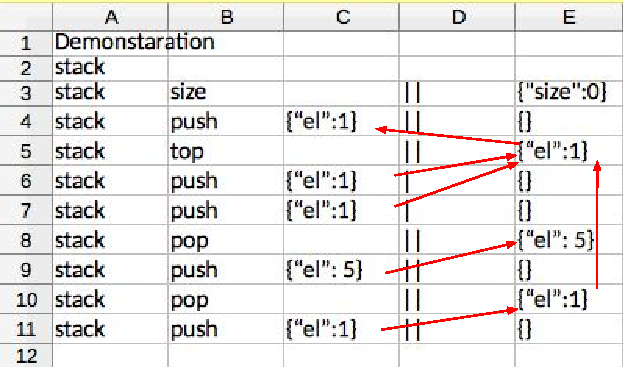
\includegraphics[width=\linewidth]{grafiken/demoTS.pdf}
\caption{Test Sheet coverage for stack.js}
\label{fig:demoTS}
\end{figure}



\section{Read Stream}

This part of the system is an implementation of combining streams pattern. From the internal view it consists of two streams. First stream performs recursive search for files in a provided directory and returns array with absolute paths to them. Second stream reads content of files with \textit{xlsx} module \url{https://www.npmjs.com/package/xlsx} and meta data of the file using embedded node.js module \textit{fs} and pushes it to the up stream.

%\lstinputlisting[
%language=Javascript, numbers=left, stepnumber=5, firstnumber=1, breaklines=true, 
%basicstyle=\footnotesize,
%numberstyle=\tiny,
%caption={read\_stream.js},
%captionpos=b,
%label=demo
%]
%{code/lib/stream/readStream.js.txt}
The \textbf{function getFilesStream} creates readable stream for reading content of directory including nested directories and returns it. 
The \textbf{variable getDataStream} defined by stream in a object mode. For every file path it accepts from the down stream  checks its extensions if its .xlsx then it reads it and obtains first sheet from the book, and reads meta data of the file and pushes it to the up stream.
This two streams are piped in to combined stream using module \textit{multipipe} \url{https://www.npmjs.com/package/multipipe} and returned by the function exported by this module.
In other words, this module exports function which accepts path to the directory and returns array of deferred values each of which is a javascript object with following structure (Listing \ref{readOut})
\lstinputlisting[
language=Javascript, numbers=left, stepnumber=5, firstnumber=1, breaklines=true, 
basicstyle=\footnotesize,
numberstyle=\tiny,
caption={Read Stream Output  / Transform Stream Input JSON},
captionpos=b,
label=readOut
]
{code/readOut.js.txt}

\subsection{Test Coverage}
Following test cases can show each step incrementally performed during the develop process. All calls to systems I/O (e. g. read file meta data, read file) are implemented using stubs. \textbf{Stub} is an implementation of \textit{proxy pattern} which allows to redefine functions behavior. This gives an opportunity to improve speed of tests by replacing functions with call to I/O with empty functions.
%\lstinputlisting[
%language=Javascript, numbers=left, stepnumber=5, firstnumber=1, breaklines=true, 
%basicstyle=\footnotesize,
%numberstyle=\tiny,
%caption={Test coverage for read\_stream.js},
%captionpos=b,
%label=readTest
%]
%{code/test/readStream.js.txt}

The result of tests execution  for this module is following (Fig.: \ref{fig:testRead}):
\begin{figure}[H]
	\centering
	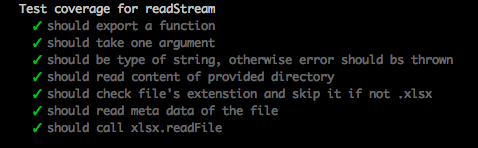
\includegraphics[width=\linewidth]{grafiken/testReadStream.png}
	\caption{Test coverage for read\_stream.js}
	\label{fig:testRead}
\end{figure}



%\paragraph{Correspondence to design principles:}
%\begin{itemize}
%	\item Closing - stream is closed over file extension, schema\_maker - object structure returned by 	\textit{xlsx} library;
%	\item Code to Interface - stream obtains and returns values via standard stream interface, call to file system made via standard nodeJS File System stream interface;
%	\item Do not Repeat Yourself - no code duplication;
%	\item Single Responsibility Principle - can be changed only due to the change of input type;
%	\item Open Close Principle - new pipes can be added in a single place;
%	\item Liscov Substitution Principle - no inherited objects used;
%	\item Interface Segregation Principle - no dependency on redundant methods;
%	\item Dependency Inversion Principle - higher level module index.js does not depend on current library
%	\item Least Knowledge Principle - communication to interfaces and invocation of used library;
%	\item Loose Coupling Principle - standard interfaces;
%\end{itemize}
%
%\textbf{Design principles implication:}
%\begin{itemize}
%\item  S. - Single Responsibility Principle - can be changed only due to the change of input type
%\item  O. - Open Close Principle - new pipes can be added in a single place
%\item  L. - Liscov Substitution Principle - no inheritance
%\item  I. - Interface Segregation Principle - Stream interface / File System interface
%\item  D. - Dependency Inversion Principle - Higgher level module index.js does not depend on current library
%
%Writer structure:\\


\section{Transform Stream}
This part of the system performs translation of the Test Sheet in to executable javascript code. In this realization of the Test Sheet concept translation performed in a two stages. The first stage necessary for the translation in a creation of \textit{schema} object of the Test Sheet. The second stage is an application of a template to the content of Test Sheet together with the file name of the xlsx file and schema created on a previous stage. The result of this transformation is pulled by the downstream as a \textit{content} property of an object together with \textit{meta data} and \textit{fileName} obtained from the upstream (Listing: \ref{writeIn}).

\lstinputlisting[
language=Javascript, numbers=left, stepnumber=5, firstnumber=1, breaklines=true, 
basicstyle=\footnotesize,
numberstyle=\tiny,
caption={Transform Stream Output / Write Stream Input JSON},
captionpos=b,
label=writeIn
]
{code/writeIn.js.txt}

\subsection{Test Coverage}
Following test cases can show each step incrementally performed during the develop process. All calls to systems I/O (e. g. read file meta data, read file) are implemented using stubs. \textbf{Stub} is an implementation of \textit{proxy pattern} which allows to redefine functions behavior. This gives an opportunity to improve speed of tests by replacing functions with call to I/O with empty functions.
%\lstinputlisting[
%language=Javascript, numbers=left, stepnumber=5, firstnumber=1, breaklines=true, 
%basicstyle=\footnotesize,
%numberstyle=\tiny,
%caption={Test coverage for transform\_stream.js },
%captionpos=b,
%label=writeIn
%]
%{code/lib/stream/transformStream.js.txt}

The result of test execution:
\begin{figure}[H]
	\centering
	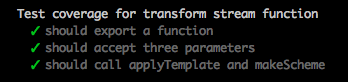
\includegraphics[width=\linewidth]{grafiken/testTransform.png}
	\caption{Test coverage for transform\_stream.js}
	\label{fig:testTransofm}
\end{figure}


\section{Schema}
This part of the system creates a schema object from the Test Sheet object, the only parameter accepted by the main function of this module. Due to the structure of object  returned after reading of xlsx file was taken decision to perform creation of the schema in two stages.

The \textbf{first stage} is creation of javascript object with Test Sheet properties (e. g. \textit{description, moduleUnderTest, objectsUnderTest, methodsUnderTest, inputs, outputs, invocations}) value of each property except \textit{description} and \textit{moduleUnderTest} are arrays of string with values which represent cell addresses for representative property of the Test Sheet. For first two properties the values are strings with values (in a Test Sheet) from the cells \textit{A1} and \textit{A2} respectively(Listing: \ref{firstScheme}).

\lstinputlisting[
language=Javascript, numbers=left, stepnumber=5, firstnumber=1, breaklines=true, 
basicstyle=\footnotesize,
numberstyle=\tiny,
caption={Result of the first stage of Test Sheet scheme creation},
captionpos=b,
label=firstScheme
]
{code/firstSchema.js.txt}

The \textbf{sectod stage} is a pivot transformation of scheme provided by the result of previous stage. Result of this stage is an object with properties  as a numbers of rows in the Test Sheet object. The values for first and second properties are values of \textit{description} and \textit{module} under test from the respective Test Sheet. While all next are objects which consists of Test Sheet following properties: \textit{objectUnderTest, methodUnderTest, inputs, outputs, invocations}. With values as single element arrays with coordinate of respective cell (Listing \ref{scheme}).
\lstinputlisting[
language=Javascript, numbers=left, stepnumber=5, firstnumber=1, breaklines=true, 
basicstyle=\footnotesize,
numberstyle=\tiny,
caption={Result of the scheme creation  for Test Sheet},
captionpos=b,
label=scheme
]
{code/scheme.js.txt}

%\lstinputlisting[
%language=Javascript, numbers=left, stepnumber=5, firstnumber=1, breaklines=true, 
%basicstyle=\footnotesize,
%numberstyle=\tiny,
%caption={Module for creation of the Test Sheet scheme},
%captionpos=b,
%label=writeIn
%]
%{code/lib/scheme/index.js.txt}
\subsection{Test Coverage}
Following test cases can show each step incrementally performed during the develop process. All calls to systems I/O (e. g. read file meta data, read file) are implemented using stubs. \textbf{Stub} is an implementation of \textit{proxy pattern} which allows to redefine functions behavior. This gives an opportunity to improve speed of tests by replacing functions with call to I/O with empty functions.
%\lstinputlisting[
%language=Javascript, numbers=left, stepnumber=5, firstnumber=1, breaklines=true, 
%basicstyle=\footnotesize,
%numberstyle=\tiny,
%caption={Test coverage for creation of the Test Sheet scheme},
%captionpos=b,
%label=writeIn
%]
%{code/test/scheme.js.txt}

The result of test execution:
\begin{figure}[H]
	\centering
	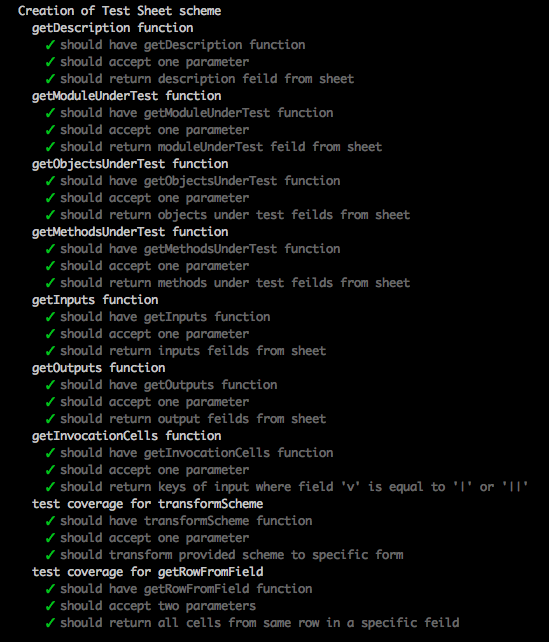
\includegraphics[width=\linewidth]{grafiken/testScheme.png}
	\caption{Test coverage for scheme.js}
	\label{fig:testScheme}
\end{figure}

\section{Execution Order}
\lstinputlisting[
language=Javascript, numbers=left, stepnumber=5, firstnumber=1, breaklines=true, 
basicstyle=\footnotesize,
numberstyle=\tiny,
caption={Result of the scheme creation  for Test Sheet},
captionpos=b,
label=scheme
]
{code/executionOrderSchema.js.txt}
\subsection{Test coverage}

\section{Execution Schema}
\lstinputlisting[
language=Javascript, numbers=left, stepnumber=5, firstnumber=1, breaklines=true, 
basicstyle=\footnotesize,
numberstyle=\tiny,
caption={Result of the scheme creation  for Test Sheet},
captionpos=b,
label=scheme
]
{code/executionSchema.js.txt}
\subsection{Test Coverage}


\section{Template}
The translation itself made by apply template function. This function accepts three parameters \textit{sheet <Object>, scheme <Object>, fileName<String>}. \textit{Sheet} is a javascript object returned by reading the content of Test Sheet file. \textit{fileName} is a absolute path to the TestSheet file. This function creates a string content for javascript file based on provided parameters. The creation takes part in a four stages. 

The \textbf{first stage} is adding a description from the first element of the scheme object. It enclosed within the multiline comment symbols.

The \textbf{second stage} is adding require of reporting module for representation of execution of the tests result.
The \textbf{third stage} is adding declarations of the module scope variables. The variable names are taken from the coordinates of cells which store input and output parameters in a Test Sheet. The values of this variables are taken as from the cells with respective addresses.
The \textbf{fourth stage} is adding calls of the methods (Listing: \ref{template}). This stage is the most important part of this module. It is implemented as \textit{addCalls} function. This is recursive function which accepts four parameter: \textit{sheet, scheme, indentation, accumulator, fileName}. First two parameters are necessary to access the values represented in a Test Sheet. Next parameter is an indentation level which represents the deepness of a function call by adding representative amount of spaces for each line of generated code. Accumulator parameter is a string to which will be appended result of each recursive call of the function. The last parameter is necessary for report mechanism which allows to record result of the test execution to appropriate file. The report mechanism (e.g \textit{makeComparisonAndWriteResult}) will be described in details within  the next section. However it is important to mention here how it works as a 'black box'. It is binary function which accepts  six parameters. First parameter is an expected return value. Second is an actual returned value received by the callback function, third is a deepness of comparison will be performed for this their values. The function returns \textbf{true} in case of match and after redefinition of the variable takes place. This mechanism allows usage of references within the Test Sheet for asynchronous functions.
\lstinputlisting[
language=Javascript, numbers=left, stepnumber=5, firstnumber=1, breaklines=true, 
basicstyle=\footnotesize,
numberstyle=\tiny,
caption={Function addCalls from template module},
captionpos=b,
label=template
]
{code/lib/template/template.js.txt}

Note that functions in the generated code are not called directly but via \textit{call} method of the function's prototype. This method provides an opportunity to call the function from different context (environment). In current example the implementation of \textit{stack} module does not depend on the environment in which it was called. But in some cases the result of function's invocation can depend on the environment in which it was invoked. One of such cases can be creation of child process, when it is necessary to provide environment manually. 


\subsection{Test Coverage}
Following test cases can show each step incrementally performed during the develop process. All calls to systems I/O (e. g. read file meta data, read file) are implemented using stubs. \textbf{Stub} is an implementation of \textit{proxy pattern} which allows to redefine functions behavior. This gives an opportunity to improve speed of tests by replacing functions with call to I/O with empty functions.

%\lstinputlisting[
%language=Javascript, numbers=left, stepnumber=5, firstnumber=1, breaklines=true, 
%basicstyle=\footnotesize,
%numberstyle=\tiny,
%caption={Test coverage for creation of the Test Sheet template},
%captionpos=b,
%label=writeIn
%]
%{code/test/template.js.txt}

The result of test execution:
\begin{figure}[H]
	\centering
	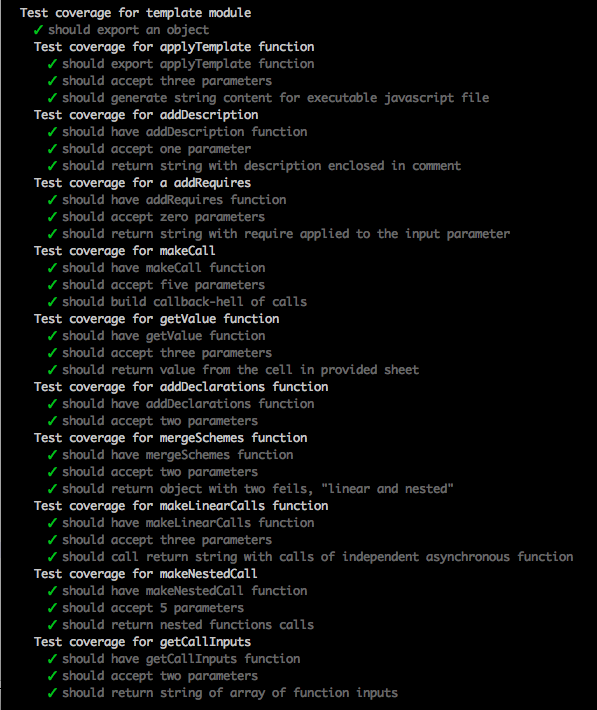
\includegraphics[width=\linewidth]{grafiken/testTemplate.png}
	\caption{Test coverage for template.js}
	\label{fig:testTemplate}
\end{figure}


\section{Write Stream}

This part of the system implements on function and exports it wrapped in to object stream. It receives an object from the up stream with following structure (Lisitng: \ref{writeIn}). It tries to read meta data of the file with same name as Test Sheet file but with the .js extension, it possible only if the file exists. In other case, the exception will be thrown and caught by catch block which implements creation of the file with content received from the up stream, and notification of user about successfully created file via standard system output or an error if the file failed to create. If file already exists the function will be able to read its meta data. After it, this meta data will be compared with meta data of the Test Sheet file received from the upstream. In case if modification date of the Test Sheet file is bigger then modification data of javascript file system will overwrite the javascript file with content received from the upstream. In other case case (Tests sheet file was not updated after creation of representative javascript file) the system will switch to the next object received from the up stream. The result javascript file generated from the provided Test Sheet looks as following (Listing: \ref{demo})

\lstinputlisting[
language=Javascript, numbers=left, stepnumber=5, firstnumber=1, breaklines=true, 
basicstyle=\footnotesize,
numberstyle=\tiny,
caption={Generated javascript file},
captionpos=b,
label=demo
]
{code/demo/demo.js.txt}

Note that functions are not called directly but via \textit{call} method.

%\lstinputlisting[
%language=Javascript, numbers=left, stepnumber=5, firstnumber=1, breaklines=true, 
%basicstyle=\footnotesize,
%numberstyle=\tiny,
%caption={write\_stream.js},
%captionpos=b,
%label=demo
%]
%{code/lib/stream/writeStream.js.txt}

\subsection{Test Coverage}
Following test cases can show each step incrementally performed during the develop process. All calls to systems I/O (e. g. read file meta data, read file) are implemented using stubs.
%\lstinputlisting[
%language=Javascript, numbers=left, stepnumber=5, firstnumber=1, breaklines=true, 
%basicstyle=\footnotesize,
%numberstyle=\tiny,
%caption={Test coverage for write\_stream.js},
%captionpos=b,
%label=writeTest
%]
%{code/test/writeStream.js.txt}


The result of tests execution  for this module is following (Fig.: \ref{fig:testWrite}): 
\begin{figure}[H]
	\centering
	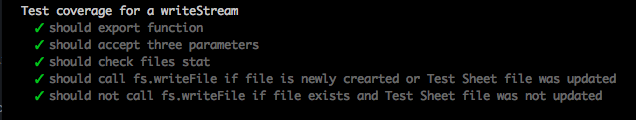
\includegraphics[width=\linewidth]{grafiken/testWriteStream.png}
	\caption{Test coverage for write\_stream.js}
	\label{fig:testWrite}
\end{figure}

\section{Reporting mechanism}
The reporting mechanism made as a standalone npm package which must me installed globally for being available at any place of the system where it is called by generated javascript files described in a previous section. 
The folder/file structure of the application looks as following:
\begin{itemize}
	\item index.js
	\item package.json
	\item ReadMe.md
	\item lib/
	\begin{itemize}
		\item compare\_and\_write.js
	\end{itemize}
	\item test/
	\begin{itemize}
		\item compare\_and\_write.js
	\end{itemize}
	\item node\_modules/
\end{itemize}

\subsection{Implementation}
\lstinputlisting[
language=Javascript, numbers=left, stepnumber=5, firstnumber=1, breaklines=true, 
basicstyle=\footnotesize,
numberstyle=\tiny,
caption={Report mechanism's main function},
captionpos=b,
label=report
]
{code/report.js.txt}

\begin{figure}[H]
	\centering
	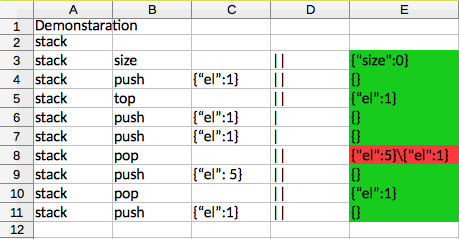
\includegraphics[width=\linewidth]{grafiken/testSheetResult.png}
	\caption{Result Test Sheet for stack.js}
	\label{fig:resultTestSheet}
\end{figure}


\subsection{Test coverage}
Following test cases can show each step incrementally performed during the develop process. All calls to systems I/O (e. g. read file meta data, read file) are implemented using stubs.
The result of tests execution  for this module is following (Fig.: \ref{fig:testReport}): 
\begin{figure}[H]
	\centering
	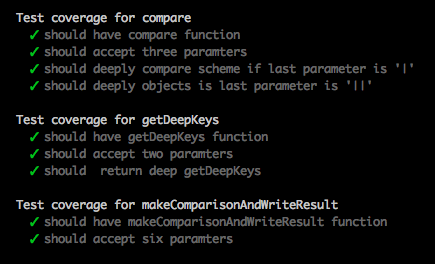
\includegraphics[width=\linewidth]{grafiken/testReport.png}
	\caption{Test coverage for report mechanism}
	\label{fig:testReport}
\end{figure}

